\documentclass[twoside]{book}

% Packages required by doxygen
\usepackage{fixltx2e}
\usepackage{calc}
\usepackage{doxygen}
\usepackage[export]{adjustbox} % also loads graphicx
\usepackage{graphicx}
\usepackage[utf8]{inputenc}
\usepackage{makeidx}
\usepackage{multicol}
\usepackage{multirow}
\PassOptionsToPackage{warn}{textcomp}
\usepackage{textcomp}
\usepackage[nointegrals]{wasysym}
\usepackage[table]{xcolor}

% NLS support packages
\usepackage[spanish]{babel}
% Font selection
\usepackage[T1]{fontenc}
\usepackage[scaled=.90]{helvet}
\usepackage{courier}
\usepackage{amssymb}
\usepackage{sectsty}
\renewcommand{\familydefault}{\sfdefault}
\allsectionsfont{%
  \fontseries{bc}\selectfont%
  \color{darkgray}%
}
\renewcommand{\DoxyLabelFont}{%
  \fontseries{bc}\selectfont%
  \color{darkgray}%
}
\newcommand{\+}{\discretionary{\mbox{\scriptsize$\hookleftarrow$}}{}{}}

% Page & text layout
\usepackage{geometry}
\geometry{%
  a4paper,%
  top=2.5cm,%
  bottom=2.5cm,%
  left=2.5cm,%
  right=2.5cm%
}
\tolerance=750
\hfuzz=15pt
\hbadness=750
\setlength{\emergencystretch}{15pt}
\setlength{\parindent}{0cm}
\setlength{\parskip}{0.2cm}
\makeatletter
\renewcommand{\paragraph}{%
  \@startsection{paragraph}{4}{0ex}{-1.0ex}{1.0ex}{%
    \normalfont\normalsize\bfseries\SS@parafont%
  }%
}
\renewcommand{\subparagraph}{%
  \@startsection{subparagraph}{5}{0ex}{-1.0ex}{1.0ex}{%
    \normalfont\normalsize\bfseries\SS@subparafont%
  }%
}
\makeatother

% Headers & footers
\usepackage{fancyhdr}
\pagestyle{fancyplain}
\fancyhead[LE]{\fancyplain{}{\bfseries\thepage}}
\fancyhead[CE]{\fancyplain{}{}}
\fancyhead[RE]{\fancyplain{}{\bfseries\leftmark}}
\fancyhead[LO]{\fancyplain{}{\bfseries\rightmark}}
\fancyhead[CO]{\fancyplain{}{}}
\fancyhead[RO]{\fancyplain{}{\bfseries\thepage}}
\fancyfoot[LE]{\fancyplain{}{}}
\fancyfoot[CE]{\fancyplain{}{}}
\fancyfoot[RE]{\fancyplain{}{\bfseries\scriptsize Generado el Miércoles, 24 de Febrero de 2016 22\+:29\+:00 para documentacion\+\_\+doxygen por Doxygen }}
\fancyfoot[LO]{\fancyplain{}{\bfseries\scriptsize Generado el Miércoles, 24 de Febrero de 2016 22\+:29\+:00 para documentacion\+\_\+doxygen por Doxygen }}
\fancyfoot[CO]{\fancyplain{}{}}
\fancyfoot[RO]{\fancyplain{}{}}
\renewcommand{\footrulewidth}{0.4pt}
\renewcommand{\chaptermark}[1]{%
  \markboth{#1}{}%
}
\renewcommand{\sectionmark}[1]{%
  \markright{\thesection\ #1}%
}

% Indices & bibliography
\usepackage{natbib}
\usepackage[titles]{tocloft}
\setcounter{tocdepth}{3}
\setcounter{secnumdepth}{5}
\makeindex

% Hyperlinks (required, but should be loaded last)
\usepackage{ifpdf}
\ifpdf
  \usepackage[pdftex,pagebackref=true]{hyperref}
\else
  \usepackage[ps2pdf,pagebackref=true]{hyperref}
\fi
\hypersetup{%
  colorlinks=true,%
  linkcolor=blue,%
  citecolor=blue,%
  unicode%
}

% Custom commands
\newcommand{\clearemptydoublepage}{%
  \newpage{\pagestyle{empty}\cleardoublepage}%
}


%===== C O N T E N T S =====

\begin{document}

% Titlepage & ToC
\hypersetup{pageanchor=false,
             bookmarks=true,
             bookmarksnumbered=true,
             pdfencoding=unicode
            }
\pagenumbering{roman}
\begin{titlepage}
\vspace*{7cm}
\begin{center}%
{\Large documentacion\+\_\+doxygen }\\
\vspace*{1cm}
{\large Generado por Doxygen 1.8.9.1}\\
\vspace*{0.5cm}
{\small Miércoles, 24 de Febrero de 2016 22:29:00}\\
\end{center}
\end{titlepage}
\clearemptydoublepage
\tableofcontents
\clearemptydoublepage
\pagenumbering{arabic}
\hypersetup{pageanchor=true}

%--- Begin generated contents ---
\chapter{Indice jerárquico}
\section{Class Hierarchy}
This inheritance list is sorted roughly, but not completely, alphabetically\+:\begin{DoxyCompactList}
\item \contentsline{section}{Practica4.\+Arbitro}{\pageref{class_practica4_1_1_arbitro}}{}
\item \contentsline{section}{Practica4.\+Pelota}{\pageref{class_practica4_1_1_pelota}}{}
\item Runnable\begin{DoxyCompactList}
\item \contentsline{section}{Practica4.\+Jugador}{\pageref{class_practica4_1_1_jugador}}{}
\end{DoxyCompactList}
\end{DoxyCompactList}

\chapter{Índice de clases}
\section{Lista de clases}
Lista de las clases, estructuras, uniones e interfaces con una breve descripción\+:\begin{DoxyCompactList}
\item\contentsline{section}{\hyperlink{class_ejercicio1__3__3_1_1_detener___interrupcion}{Ejercicio1\+\_\+3\+\_\+3.\+Detener\+\_\+\+Interrupcion} \\*Thread que se detiene tras una señal del usuario, con diferentes acciones en función del tiempo transcurrido }{\pageref{class_ejercicio1__3__3_1_1_detener___interrupcion}}{}
\item\contentsline{section}{\hyperlink{class_ejercicio1__2__1_1_1_ejercicio1}{Ejercicio1\+\_\+2\+\_\+1.\+Ejercicio1} \\*Creación del número de hilos especificados por el usuario }{\pageref{class_ejercicio1__2__1_1_1_ejercicio1}}{}
\item\contentsline{section}{\hyperlink{class_ejercicio1__2__1_1_1_ejercicio2}{Ejercicio1\+\_\+2\+\_\+1.\+Ejercicio2} \\*Creación del número de hilos especificados por el usuario y medición del tiempo de ejecucion de los hilos }{\pageref{class_ejercicio1__2__1_1_1_ejercicio2}}{}
\item\contentsline{section}{\hyperlink{class_ejercicio1__2__4_1_1_ejercicio4}{Ejercicio1\+\_\+2\+\_\+4.\+Ejercicio4} \\*Cada thread calcula su tiempo de ejecución, lo almacena en una variable publica y se calcula el tiempo total }{\pageref{class_ejercicio1__2__4_1_1_ejercicio4}}{}
\item\contentsline{section}{\hyperlink{class_ejercicio1__2__5_1_1_ejercicio5}{Ejercicio1\+\_\+2\+\_\+5.\+Ejercicio5} \\*Muestra por separados los tiempos de inicialización de threads y los tiempos de ejecución de threads }{\pageref{class_ejercicio1__2__5_1_1_ejercicio5}}{}
\item\contentsline{section}{\hyperlink{class_ejercicio1__2__6_1_1_ejercicio6}{Ejercicio1\+\_\+2\+\_\+6.\+Ejercicio6} \\*Al crear los threads, en caso de introducir el valor \char`\"{}1\char`\"{} se realiza una operación compleja, en caso contrario se procede a la identificación finalización de los threads }{\pageref{class_ejercicio1__2__6_1_1_ejercicio6}}{}
\item\contentsline{section}{\hyperlink{class_ejercicio1__1__2_1_1hello_runnable}{Ejercicio1\+\_\+1\+\_\+2.\+hello\+Runnable} \\*Creación de hilos usando la clase Runnable }{\pageref{class_ejercicio1__1__2_1_1hello_runnable}}{}
\item\contentsline{section}{\hyperlink{class_ejercicio1__1__3_1_1hello_runnable___sleep}{Ejercicio1\+\_\+1\+\_\+3.\+hello\+Runnable\+\_\+\+Sleep} \\*Creación de hilos usando la clase Runnable y usando el método sleep para crear el delay de 1 segundo }{\pageref{class_ejercicio1__1__3_1_1hello_runnable___sleep}}{}
\item\contentsline{section}{\hyperlink{class_ejercicio1__1__2_1_1hello_thread}{Ejercicio1\+\_\+1\+\_\+2.\+hello\+Thread} \\*Creación de hilos usando la clase Thread }{\pageref{class_ejercicio1__1__2_1_1hello_thread}}{}
\item\contentsline{section}{\hyperlink{class_ejercicio1__1__3_1_1hello_thread___sleep}{Ejercicio1\+\_\+1\+\_\+3.\+hello\+Thread\+\_\+\+Sleep} \\*Creación de hilos usando la clase Thread y usando el método sleep para crear el delay de 1 segundo }{\pageref{class_ejercicio1__1__3_1_1hello_thread___sleep}}{}
\item\contentsline{section}{\hyperlink{class_ejercicio1__1__4_1_1_runnable___activo}{Ejercicio1\+\_\+1\+\_\+4.\+Runnable\+\_\+\+Activo} \\*Creación de hilos usando la clase Runnable y usando los metodos active\+Count y current\+Thread para postrar el numero de hilos y el hilo actual }{\pageref{class_ejercicio1__1__4_1_1_runnable___activo}}{}
\item\contentsline{section}{\hyperlink{class_ejercicio1__1__4_1_1_thread___activo}{Ejercicio1\+\_\+1\+\_\+4.\+Thread\+\_\+\+Activo} \\*Creación de hilos usando la clase Thread y usando los metodos active\+Count y current\+Thread para postrar el numero de hilos y el hilo actual }{\pageref{class_ejercicio1__1__4_1_1_thread___activo}}{}
\item\contentsline{section}{\hyperlink{class_ejercicio1__3__2_1_1_thread___detenido}{Ejercicio1\+\_\+3\+\_\+2.\+Thread\+\_\+\+Detenido} \\*Crea un Thread y comprueba con is\+Interrupted() e interrupted() antes y después de interrumpirlo }{\pageref{class_ejercicio1__3__2_1_1_thread___detenido}}{}
\end{DoxyCompactList}

\chapter{Documentación de las clases}
\hypertarget{class_ejercicio1__3__3_1_1_detener___interrupcion}{}\section{Referencia de la Clase Ejercicio1\+\_\+3\+\_\+3.\+Detener\+\_\+\+Interrupcion}
\label{class_ejercicio1__3__3_1_1_detener___interrupcion}\index{Ejercicio1\+\_\+3\+\_\+3.\+Detener\+\_\+\+Interrupcion@{Ejercicio1\+\_\+3\+\_\+3.\+Detener\+\_\+\+Interrupcion}}


Thread que se detiene tras una señal del usuario, con diferentes acciones en función del tiempo transcurrido.  




Diagrama de herencias de Ejercicio1\+\_\+3\+\_\+3.\+Detener\+\_\+\+Interrupcion
\nopagebreak
\begin{figure}[H]
\begin{center}
\leavevmode
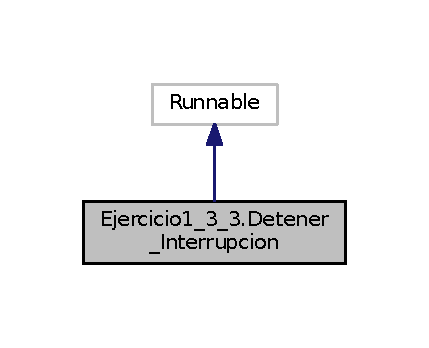
\includegraphics[width=206pt]{class_ejercicio1__3__3_1_1_detener___interrupcion__inherit__graph}
\end{center}
\end{figure}


Diagrama de colaboración para Ejercicio1\+\_\+3\+\_\+3.\+Detener\+\_\+\+Interrupcion\+:
\nopagebreak
\begin{figure}[H]
\begin{center}
\leavevmode
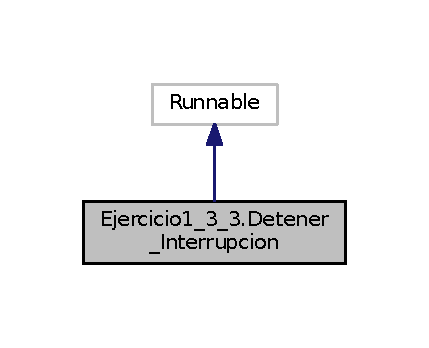
\includegraphics[width=206pt]{class_ejercicio1__3__3_1_1_detener___interrupcion__coll__graph}
\end{center}
\end{figure}
\subsection*{Métodos públicos}
\begin{DoxyCompactItemize}
\item 
\hypertarget{class_ejercicio1__3__3_1_1_detener___interrupcion_a5c76a74a9d252bcbe4598f44f5446a4b}{}void \hyperlink{class_ejercicio1__3__3_1_1_detener___interrupcion_a5c76a74a9d252bcbe4598f44f5446a4b}{run} ()\label{class_ejercicio1__3__3_1_1_detener___interrupcion_a5c76a74a9d252bcbe4598f44f5446a4b}

\begin{DoxyCompactList}\small\item\em Función run para iniciar el thread. \end{DoxyCompactList}\item 
\hypertarget{class_ejercicio1__3__3_1_1_detener___interrupcion_ab9c8bbc6ee2ecc4c65b0e5103bdeb087}{}void {\bfseries setdetener} ()\label{class_ejercicio1__3__3_1_1_detener___interrupcion_ab9c8bbc6ee2ecc4c65b0e5103bdeb087}

\end{DoxyCompactItemize}
\subsection*{Métodos públicos estáticos}
\begin{DoxyCompactItemize}
\item 
static void \hyperlink{class_ejercicio1__3__3_1_1_detener___interrupcion_adfc3aa05263913c292052bc839e8ad97}{main} (String\mbox{[}$\,$\mbox{]} args)
\begin{DoxyCompactList}\small\item\em Función main del ejercicio. \end{DoxyCompactList}\end{DoxyCompactItemize}


\subsection{Descripción detallada}
Thread que se detiene tras una señal del usuario, con diferentes acciones en función del tiempo transcurrido. 

\begin{DoxyAuthor}{Autor}
Nara, Javier, Esteban 
\end{DoxyAuthor}


\subsection{Documentación de las funciones miembro}
\hypertarget{class_ejercicio1__3__3_1_1_detener___interrupcion_adfc3aa05263913c292052bc839e8ad97}{}\index{Ejercicio1\+\_\+3\+\_\+3\+::\+Detener\+\_\+\+Interrupcion@{Ejercicio1\+\_\+3\+\_\+3\+::\+Detener\+\_\+\+Interrupcion}!main@{main}}
\index{main@{main}!Ejercicio1\+\_\+3\+\_\+3\+::\+Detener\+\_\+\+Interrupcion@{Ejercicio1\+\_\+3\+\_\+3\+::\+Detener\+\_\+\+Interrupcion}}
\subsubsection[{main}]{\setlength{\rightskip}{0pt plus 5cm}static void Ejercicio1\+\_\+3\+\_\+3.\+Detener\+\_\+\+Interrupcion.\+main (
\begin{DoxyParamCaption}
\item[{String\mbox{[}$\,$\mbox{]}}]{args}
\end{DoxyParamCaption}
)\hspace{0.3cm}{\ttfamily [static]}}\label{class_ejercicio1__3__3_1_1_detener___interrupcion_adfc3aa05263913c292052bc839e8ad97}


Función main del ejercicio. 

Función main del ejercicio 

La documentación para esta clase fue generada a partir del siguiente fichero\+:\begin{DoxyCompactItemize}
\item 
Ejercicio1\+\_\+3\+\_\+3/Detener\+\_\+\+Interrupcion.\+java\end{DoxyCompactItemize}

\hypertarget{class_ejercicio1__2__1_1_1_ejercicio1}{}\section{Referencia de la Clase Ejercicio1\+\_\+2\+\_\+1.\+Ejercicio1}
\label{class_ejercicio1__2__1_1_1_ejercicio1}\index{Ejercicio1\+\_\+2\+\_\+1.\+Ejercicio1@{Ejercicio1\+\_\+2\+\_\+1.\+Ejercicio1}}


Creación del número de hilos especificados por el usuario.  




Diagrama de herencias de Ejercicio1\+\_\+2\+\_\+1.\+Ejercicio1
\nopagebreak
\begin{figure}[H]
\begin{center}
\leavevmode
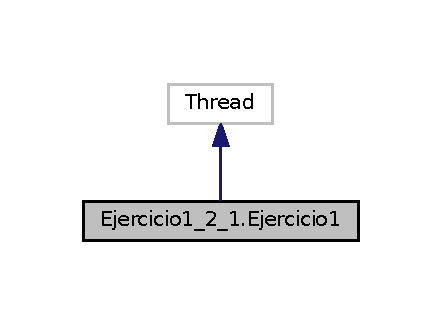
\includegraphics[width=212pt]{class_ejercicio1__2__1_1_1_ejercicio1__inherit__graph}
\end{center}
\end{figure}


Diagrama de colaboración para Ejercicio1\+\_\+2\+\_\+1.\+Ejercicio1\+:
\nopagebreak
\begin{figure}[H]
\begin{center}
\leavevmode
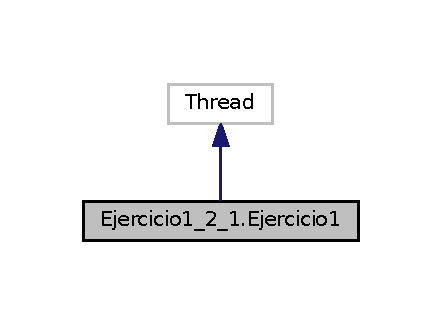
\includegraphics[width=212pt]{class_ejercicio1__2__1_1_1_ejercicio1__coll__graph}
\end{center}
\end{figure}
\subsection*{Métodos públicos}
\begin{DoxyCompactItemize}
\item 
\hypertarget{class_ejercicio1__2__1_1_1_ejercicio1_ad1f2c70cdbcba131faafb12f2dd15db2}{}{\bfseries Ejercicio1} (int n)\label{class_ejercicio1__2__1_1_1_ejercicio1_ad1f2c70cdbcba131faafb12f2dd15db2}

\item 
\hypertarget{class_ejercicio1__2__1_1_1_ejercicio1_a859e2a8b18a0a631b83828af1bd55de4}{}void \hyperlink{class_ejercicio1__2__1_1_1_ejercicio1_a859e2a8b18a0a631b83828af1bd55de4}{run} ()\label{class_ejercicio1__2__1_1_1_ejercicio1_a859e2a8b18a0a631b83828af1bd55de4}

\begin{DoxyCompactList}\small\item\em Función run para iniciar el thread. \end{DoxyCompactList}\end{DoxyCompactItemize}
\subsection*{Métodos públicos estáticos}
\begin{DoxyCompactItemize}
\item 
\hypertarget{class_ejercicio1__2__1_1_1_ejercicio1_a2e65f0073f5378723ce1c4869865124c}{}static void \hyperlink{class_ejercicio1__2__1_1_1_ejercicio1_a2e65f0073f5378723ce1c4869865124c}{main} (String\mbox{[}$\,$\mbox{]} args)\label{class_ejercicio1__2__1_1_1_ejercicio1_a2e65f0073f5378723ce1c4869865124c}

\begin{DoxyCompactList}\small\item\em Función main del ejercicio. \end{DoxyCompactList}\end{DoxyCompactItemize}


\subsection{Descripción detallada}
Creación del número de hilos especificados por el usuario. 

\begin{DoxyAuthor}{Autor}
Nara, Javier, Esteban 
\end{DoxyAuthor}


La documentación para esta clase fue generada a partir del siguiente fichero\+:\begin{DoxyCompactItemize}
\item 
Ejercicio1\+\_\+2\+\_\+1/Ejercicio1.\+java\end{DoxyCompactItemize}

\hypertarget{class_ejercicio1__2__1_1_1_ejercicio2}{}\section{Referencia de la Clase Ejercicio1\+\_\+2\+\_\+1.\+Ejercicio2}
\label{class_ejercicio1__2__1_1_1_ejercicio2}\index{Ejercicio1\+\_\+2\+\_\+1.\+Ejercicio2@{Ejercicio1\+\_\+2\+\_\+1.\+Ejercicio2}}


Creación del número de hilos especificados por el usuario y medición del tiempo de ejecucion de los hilos.  




Diagrama de herencias de Ejercicio1\+\_\+2\+\_\+1.\+Ejercicio2
\nopagebreak
\begin{figure}[H]
\begin{center}
\leavevmode
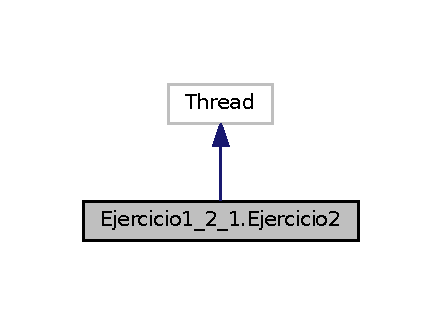
\includegraphics[width=212pt]{class_ejercicio1__2__1_1_1_ejercicio2__inherit__graph}
\end{center}
\end{figure}


Diagrama de colaboración para Ejercicio1\+\_\+2\+\_\+1.\+Ejercicio2\+:
\nopagebreak
\begin{figure}[H]
\begin{center}
\leavevmode
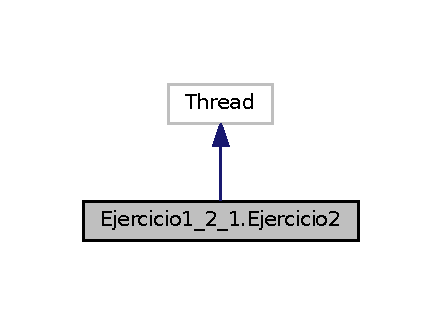
\includegraphics[width=212pt]{class_ejercicio1__2__1_1_1_ejercicio2__coll__graph}
\end{center}
\end{figure}
\subsection*{Métodos públicos}
\begin{DoxyCompactItemize}
\item 
\hypertarget{class_ejercicio1__2__1_1_1_ejercicio2_aebfccde0e9e4f76521e85b253966a1aa}{}{\bfseries Ejercicio2} (int n)\label{class_ejercicio1__2__1_1_1_ejercicio2_aebfccde0e9e4f76521e85b253966a1aa}

\item 
\hypertarget{class_ejercicio1__2__1_1_1_ejercicio2_a2c66ccaa4198d9a0834977d21171a801}{}void \hyperlink{class_ejercicio1__2__1_1_1_ejercicio2_a2c66ccaa4198d9a0834977d21171a801}{run} ()\label{class_ejercicio1__2__1_1_1_ejercicio2_a2c66ccaa4198d9a0834977d21171a801}

\begin{DoxyCompactList}\small\item\em Función run para iniciar el thread. \end{DoxyCompactList}\end{DoxyCompactItemize}
\subsection*{Métodos públicos estáticos}
\begin{DoxyCompactItemize}
\item 
\hypertarget{class_ejercicio1__2__1_1_1_ejercicio2_a8b28d2e41a5e7e08e7024df7f8967b0b}{}static void \hyperlink{class_ejercicio1__2__1_1_1_ejercicio2_a8b28d2e41a5e7e08e7024df7f8967b0b}{main} (String\mbox{[}$\,$\mbox{]} args)\label{class_ejercicio1__2__1_1_1_ejercicio2_a8b28d2e41a5e7e08e7024df7f8967b0b}

\begin{DoxyCompactList}\small\item\em Función main del ejercicio. \end{DoxyCompactList}\end{DoxyCompactItemize}


\subsection{Descripción detallada}
Creación del número de hilos especificados por el usuario y medición del tiempo de ejecucion de los hilos. 

\begin{DoxyAuthor}{Autor}
Nara, Javier, Esteban 
\end{DoxyAuthor}


La documentación para esta clase fue generada a partir del siguiente fichero\+:\begin{DoxyCompactItemize}
\item 
Ejercicio1\+\_\+2\+\_\+2/Ejercicio2.\+java\end{DoxyCompactItemize}

\hypertarget{class_ejercicio1__2__4_1_1_ejercicio4}{}\section{Referencia de la Clase Ejercicio1\+\_\+2\+\_\+4.\+Ejercicio4}
\label{class_ejercicio1__2__4_1_1_ejercicio4}\index{Ejercicio1\+\_\+2\+\_\+4.\+Ejercicio4@{Ejercicio1\+\_\+2\+\_\+4.\+Ejercicio4}}


Cada thread calcula su tiempo de ejecución, lo almacena en una variable publica y se calcula el tiempo total.  




Diagrama de herencias de Ejercicio1\+\_\+2\+\_\+4.\+Ejercicio4
\nopagebreak
\begin{figure}[H]
\begin{center}
\leavevmode
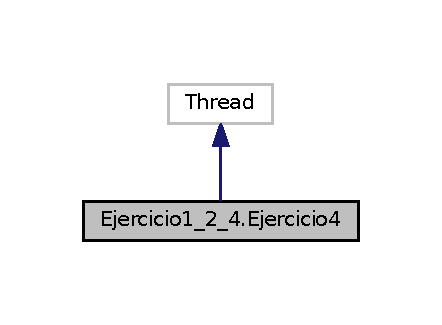
\includegraphics[width=212pt]{class_ejercicio1__2__4_1_1_ejercicio4__inherit__graph}
\end{center}
\end{figure}


Diagrama de colaboración para Ejercicio1\+\_\+2\+\_\+4.\+Ejercicio4\+:
\nopagebreak
\begin{figure}[H]
\begin{center}
\leavevmode
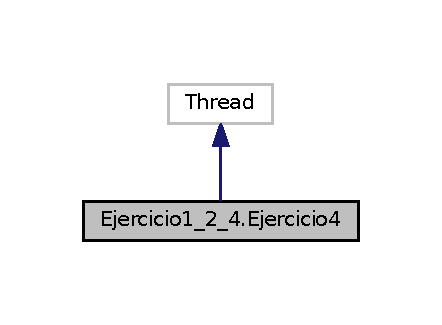
\includegraphics[width=212pt]{class_ejercicio1__2__4_1_1_ejercicio4__coll__graph}
\end{center}
\end{figure}
\subsection*{Métodos públicos}
\begin{DoxyCompactItemize}
\item 
\hypertarget{class_ejercicio1__2__4_1_1_ejercicio4_aad168e519e47728e00714a20bf4e5071}{}{\bfseries Ejercicio4} (int n)\label{class_ejercicio1__2__4_1_1_ejercicio4_aad168e519e47728e00714a20bf4e5071}

\item 
\hypertarget{class_ejercicio1__2__4_1_1_ejercicio4_a650342d160590b886c63eace2388cd10}{}void \hyperlink{class_ejercicio1__2__4_1_1_ejercicio4_a650342d160590b886c63eace2388cd10}{run} ()\label{class_ejercicio1__2__4_1_1_ejercicio4_a650342d160590b886c63eace2388cd10}

\begin{DoxyCompactList}\small\item\em Función run para iniciar el thread. \end{DoxyCompactList}\end{DoxyCompactItemize}
\subsection*{Métodos públicos estáticos}
\begin{DoxyCompactItemize}
\item 
\hypertarget{class_ejercicio1__2__4_1_1_ejercicio4_ae0107d9c149901d15ff64fd908452f92}{}static void \hyperlink{class_ejercicio1__2__4_1_1_ejercicio4_ae0107d9c149901d15ff64fd908452f92}{main} (String\mbox{[}$\,$\mbox{]} args)\label{class_ejercicio1__2__4_1_1_ejercicio4_ae0107d9c149901d15ff64fd908452f92}

\begin{DoxyCompactList}\small\item\em Función main del ejercicio. \end{DoxyCompactList}\end{DoxyCompactItemize}
\subsection*{Atributos públicos}
\begin{DoxyCompactItemize}
\item 
\hypertarget{class_ejercicio1__2__4_1_1_ejercicio4_a358d67eb8478ad0a754c0f408de35bbb}{}double {\bfseries tiempo}\label{class_ejercicio1__2__4_1_1_ejercicio4_a358d67eb8478ad0a754c0f408de35bbb}

\end{DoxyCompactItemize}


\subsection{Descripción detallada}
Cada thread calcula su tiempo de ejecución, lo almacena en una variable publica y se calcula el tiempo total. 

\begin{DoxyAuthor}{Autor}
Nara, Javier, Esteban 
\end{DoxyAuthor}


La documentación para esta clase fue generada a partir del siguiente fichero\+:\begin{DoxyCompactItemize}
\item 
Ejercicio1\+\_\+2\+\_\+4/Ejercicio4.\+java\end{DoxyCompactItemize}

\hypertarget{class_ejercicio1__2__5_1_1_ejercicio5}{}\section{Referencia de la Clase Ejercicio1\+\_\+2\+\_\+5.\+Ejercicio5}
\label{class_ejercicio1__2__5_1_1_ejercicio5}\index{Ejercicio1\+\_\+2\+\_\+5.\+Ejercicio5@{Ejercicio1\+\_\+2\+\_\+5.\+Ejercicio5}}


Muestra por separados los tiempos de inicialización de threads y los tiempos de ejecución de threads.  




Diagrama de herencias de Ejercicio1\+\_\+2\+\_\+5.\+Ejercicio5
\nopagebreak
\begin{figure}[H]
\begin{center}
\leavevmode
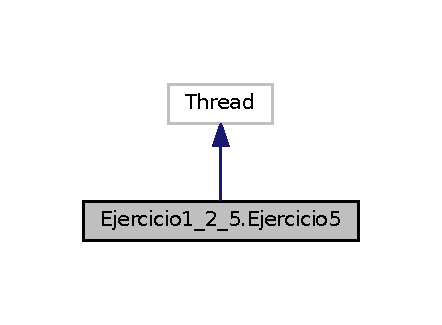
\includegraphics[width=212pt]{class_ejercicio1__2__5_1_1_ejercicio5__inherit__graph}
\end{center}
\end{figure}


Diagrama de colaboración para Ejercicio1\+\_\+2\+\_\+5.\+Ejercicio5\+:
\nopagebreak
\begin{figure}[H]
\begin{center}
\leavevmode
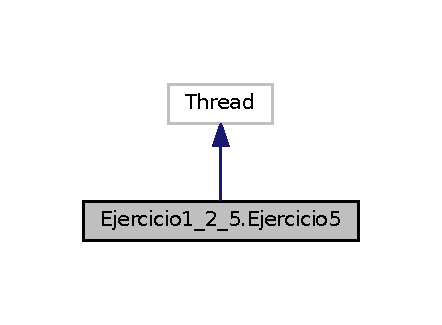
\includegraphics[width=212pt]{class_ejercicio1__2__5_1_1_ejercicio5__coll__graph}
\end{center}
\end{figure}
\subsection*{Métodos públicos}
\begin{DoxyCompactItemize}
\item 
\hypertarget{class_ejercicio1__2__5_1_1_ejercicio5_abd78f61f5410b32ef7ef1b531ea5eba7}{}{\bfseries Ejercicio5} (int n)\label{class_ejercicio1__2__5_1_1_ejercicio5_abd78f61f5410b32ef7ef1b531ea5eba7}

\item 
\hypertarget{class_ejercicio1__2__5_1_1_ejercicio5_ac2367ec1d72ad7cf755d846760af3d03}{}void \hyperlink{class_ejercicio1__2__5_1_1_ejercicio5_ac2367ec1d72ad7cf755d846760af3d03}{run} ()\label{class_ejercicio1__2__5_1_1_ejercicio5_ac2367ec1d72ad7cf755d846760af3d03}

\begin{DoxyCompactList}\small\item\em Función run para iniciar el thread. \end{DoxyCompactList}\end{DoxyCompactItemize}
\subsection*{Métodos públicos estáticos}
\begin{DoxyCompactItemize}
\item 
\hypertarget{class_ejercicio1__2__5_1_1_ejercicio5_a099d2cc93afcd8d311ef14064cf68a53}{}static void {\bfseries main} (String\mbox{[}$\,$\mbox{]} args)\label{class_ejercicio1__2__5_1_1_ejercicio5_a099d2cc93afcd8d311ef14064cf68a53}

\end{DoxyCompactItemize}


\subsection{Descripción detallada}
Muestra por separados los tiempos de inicialización de threads y los tiempos de ejecución de threads. 

\begin{DoxyAuthor}{Autor}
Nara, Javier, Esteban 
\end{DoxyAuthor}


La documentación para esta clase fue generada a partir del siguiente fichero\+:\begin{DoxyCompactItemize}
\item 
Ejercicio1\+\_\+2\+\_\+5/Ejercicio5.\+java\end{DoxyCompactItemize}

\hypertarget{class_ejercicio1__2__6_1_1_ejercicio6}{}\section{Referencia de la Clase Ejercicio1\+\_\+2\+\_\+6.\+Ejercicio6}
\label{class_ejercicio1__2__6_1_1_ejercicio6}\index{Ejercicio1\+\_\+2\+\_\+6.\+Ejercicio6@{Ejercicio1\+\_\+2\+\_\+6.\+Ejercicio6}}


Al crear los threads, en caso de introducir el valor \char`\"{}1\char`\"{} se realiza una operación compleja, en caso contrario se procede a la identificación finalización de los threads.  




Diagrama de herencias de Ejercicio1\+\_\+2\+\_\+6.\+Ejercicio6
\nopagebreak
\begin{figure}[H]
\begin{center}
\leavevmode
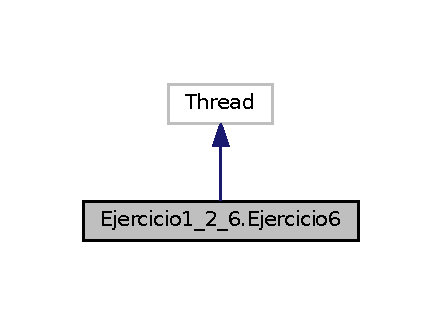
\includegraphics[width=212pt]{class_ejercicio1__2__6_1_1_ejercicio6__inherit__graph}
\end{center}
\end{figure}


Diagrama de colaboración para Ejercicio1\+\_\+2\+\_\+6.\+Ejercicio6\+:
\nopagebreak
\begin{figure}[H]
\begin{center}
\leavevmode
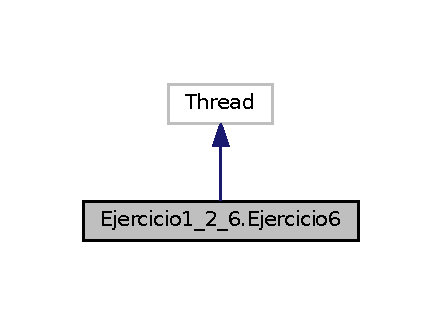
\includegraphics[width=212pt]{class_ejercicio1__2__6_1_1_ejercicio6__coll__graph}
\end{center}
\end{figure}
\subsection*{Métodos públicos}
\begin{DoxyCompactItemize}
\item 
\hypertarget{class_ejercicio1__2__6_1_1_ejercicio6_a0f26beeead5d81eeccbcb16783ab28b6}{}{\bfseries Ejercicio6} (int valor, int n)\label{class_ejercicio1__2__6_1_1_ejercicio6_a0f26beeead5d81eeccbcb16783ab28b6}

\item 
\hypertarget{class_ejercicio1__2__6_1_1_ejercicio6_a0d280114351d6076e16146dff4c95f9e}{}void \hyperlink{class_ejercicio1__2__6_1_1_ejercicio6_a0d280114351d6076e16146dff4c95f9e}{run} ()\label{class_ejercicio1__2__6_1_1_ejercicio6_a0d280114351d6076e16146dff4c95f9e}

\begin{DoxyCompactList}\small\item\em Función run para iniciar el thread. \end{DoxyCompactList}\end{DoxyCompactItemize}
\subsection*{Métodos públicos estáticos}
\begin{DoxyCompactItemize}
\item 
\hypertarget{class_ejercicio1__2__6_1_1_ejercicio6_a88527c0dfa24f4f71dabd851b69b3f4a}{}static void \hyperlink{class_ejercicio1__2__6_1_1_ejercicio6_a88527c0dfa24f4f71dabd851b69b3f4a}{main} (String\mbox{[}$\,$\mbox{]} args)  throws Interrupted\+Exception      \label{class_ejercicio1__2__6_1_1_ejercicio6_a88527c0dfa24f4f71dabd851b69b3f4a}

\begin{DoxyCompactList}\small\item\em Función main del ejercicio. \end{DoxyCompactList}\end{DoxyCompactItemize}


\subsection{Descripción detallada}
Al crear los threads, en caso de introducir el valor \char`\"{}1\char`\"{} se realiza una operación compleja, en caso contrario se procede a la identificación finalización de los threads. 

\begin{DoxyAuthor}{Autor}
Nara, Javier, Esteban 
\end{DoxyAuthor}


La documentación para esta clase fue generada a partir del siguiente fichero\+:\begin{DoxyCompactItemize}
\item 
Ejercicio1\+\_\+2\+\_\+6/Ejercicio6.\+java\end{DoxyCompactItemize}

\hypertarget{class_ejercicio1__1__2_1_1hello_runnable}{}\section{Referencia de la Clase Ejercicio1\+\_\+1\+\_\+2.\+hello\+Runnable}
\label{class_ejercicio1__1__2_1_1hello_runnable}\index{Ejercicio1\+\_\+1\+\_\+2.\+hello\+Runnable@{Ejercicio1\+\_\+1\+\_\+2.\+hello\+Runnable}}


Creación de hilos usando la clase Runnable.  




Diagrama de herencias de Ejercicio1\+\_\+1\+\_\+2.\+hello\+Runnable
\nopagebreak
\begin{figure}[H]
\begin{center}
\leavevmode
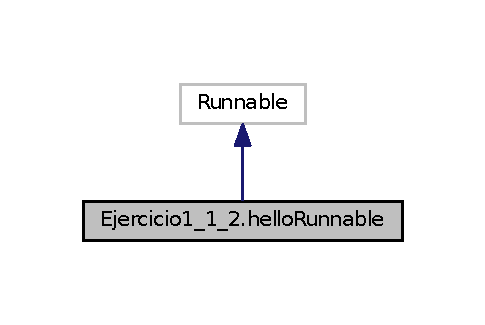
\includegraphics[width=233pt]{class_ejercicio1__1__2_1_1hello_runnable__inherit__graph}
\end{center}
\end{figure}


Diagrama de colaboración para Ejercicio1\+\_\+1\+\_\+2.\+hello\+Runnable\+:
\nopagebreak
\begin{figure}[H]
\begin{center}
\leavevmode
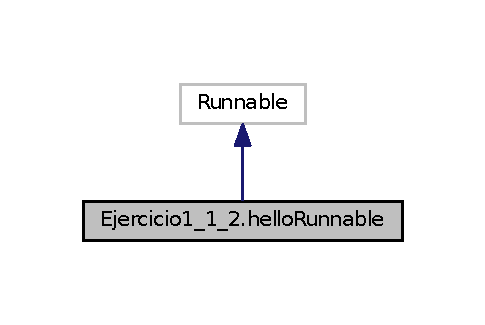
\includegraphics[width=233pt]{class_ejercicio1__1__2_1_1hello_runnable__coll__graph}
\end{center}
\end{figure}
\subsection*{Métodos públicos}
\begin{DoxyCompactItemize}
\item 
\hypertarget{class_ejercicio1__1__2_1_1hello_runnable_a27a035138d87853e1cc0d8e30c6d3dd2}{}void \hyperlink{class_ejercicio1__1__2_1_1hello_runnable_a27a035138d87853e1cc0d8e30c6d3dd2}{run} ()\label{class_ejercicio1__1__2_1_1hello_runnable_a27a035138d87853e1cc0d8e30c6d3dd2}

\begin{DoxyCompactList}\small\item\em Función run para iniciar el thread. \end{DoxyCompactList}\end{DoxyCompactItemize}
\subsection*{Métodos públicos estáticos}
\begin{DoxyCompactItemize}
\item 
\hypertarget{class_ejercicio1__1__2_1_1hello_runnable_a7e90a3111107454bc7051d2d081fb494}{}static void \hyperlink{class_ejercicio1__1__2_1_1hello_runnable_a7e90a3111107454bc7051d2d081fb494}{main} (String\mbox{[}$\,$\mbox{]} args)\label{class_ejercicio1__1__2_1_1hello_runnable_a7e90a3111107454bc7051d2d081fb494}

\begin{DoxyCompactList}\small\item\em Función main del ejercicio. \end{DoxyCompactList}\end{DoxyCompactItemize}


\subsection{Descripción detallada}
Creación de hilos usando la clase Runnable. 

\begin{DoxyAuthor}{Autor}
Nara, Javier, Esteban 
\end{DoxyAuthor}


La documentación para esta clase fue generada a partir del siguiente fichero\+:\begin{DoxyCompactItemize}
\item 
Ejercicio1\+\_\+1\+\_\+2/hello\+Runnable.\+java\end{DoxyCompactItemize}

\hypertarget{class_ejercicio1__1__3_1_1hello_runnable___sleep}{}\section{Referencia de la Clase Ejercicio1\+\_\+1\+\_\+3.\+hello\+Runnable\+\_\+\+Sleep}
\label{class_ejercicio1__1__3_1_1hello_runnable___sleep}\index{Ejercicio1\+\_\+1\+\_\+3.\+hello\+Runnable\+\_\+\+Sleep@{Ejercicio1\+\_\+1\+\_\+3.\+hello\+Runnable\+\_\+\+Sleep}}


Creación de hilos usando la clase Runnable y usando el método sleep para crear el delay de 1 segundo.  




Diagrama de herencias de Ejercicio1\+\_\+1\+\_\+3.\+hello\+Runnable\+\_\+\+Sleep
\nopagebreak
\begin{figure}[H]
\begin{center}
\leavevmode
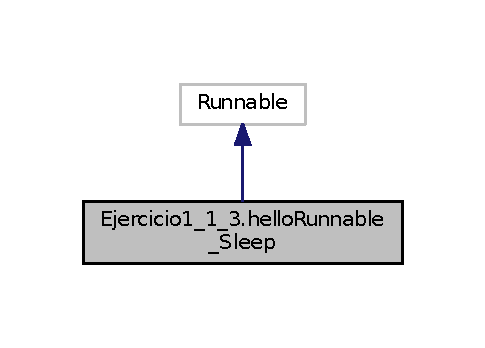
\includegraphics[width=233pt]{class_ejercicio1__1__3_1_1hello_runnable___sleep__inherit__graph}
\end{center}
\end{figure}


Diagrama de colaboración para Ejercicio1\+\_\+1\+\_\+3.\+hello\+Runnable\+\_\+\+Sleep\+:
\nopagebreak
\begin{figure}[H]
\begin{center}
\leavevmode
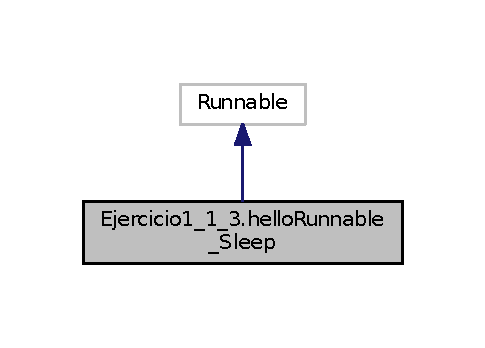
\includegraphics[width=233pt]{class_ejercicio1__1__3_1_1hello_runnable___sleep__coll__graph}
\end{center}
\end{figure}
\subsection*{Métodos públicos}
\begin{DoxyCompactItemize}
\item 
\hypertarget{class_ejercicio1__1__3_1_1hello_runnable___sleep_a6c927c4f6335ff596aeec32b5e746bd8}{}void \hyperlink{class_ejercicio1__1__3_1_1hello_runnable___sleep_a6c927c4f6335ff596aeec32b5e746bd8}{run} ()\label{class_ejercicio1__1__3_1_1hello_runnable___sleep_a6c927c4f6335ff596aeec32b5e746bd8}

\begin{DoxyCompactList}\small\item\em Función run para iniciar el thread. \end{DoxyCompactList}\end{DoxyCompactItemize}
\subsection*{Métodos públicos estáticos}
\begin{DoxyCompactItemize}
\item 
\hypertarget{class_ejercicio1__1__3_1_1hello_runnable___sleep_ac0e52a6a4f12fbede032f7b8a1224e6e}{}static void {\bfseries main} (String\mbox{[}$\,$\mbox{]} args)\label{class_ejercicio1__1__3_1_1hello_runnable___sleep_ac0e52a6a4f12fbede032f7b8a1224e6e}

\end{DoxyCompactItemize}


\subsection{Descripción detallada}
Creación de hilos usando la clase Runnable y usando el método sleep para crear el delay de 1 segundo. 

\begin{DoxyAuthor}{Autor}
Nara, Javier, Esteban 
\end{DoxyAuthor}


La documentación para esta clase fue generada a partir del siguiente fichero\+:\begin{DoxyCompactItemize}
\item 
Ejercicio1\+\_\+1\+\_\+3/hello\+Runnable\+\_\+\+Sleep.\+java\end{DoxyCompactItemize}

\hypertarget{class_ejercicio1__1__2_1_1hello_thread}{}\section{Referencia de la Clase Ejercicio1\+\_\+1\+\_\+2.\+hello\+Thread}
\label{class_ejercicio1__1__2_1_1hello_thread}\index{Ejercicio1\+\_\+1\+\_\+2.\+hello\+Thread@{Ejercicio1\+\_\+1\+\_\+2.\+hello\+Thread}}


Creación de hilos usando la clase Thread.  




Diagrama de herencias de Ejercicio1\+\_\+1\+\_\+2.\+hello\+Thread
\nopagebreak
\begin{figure}[H]
\begin{center}
\leavevmode
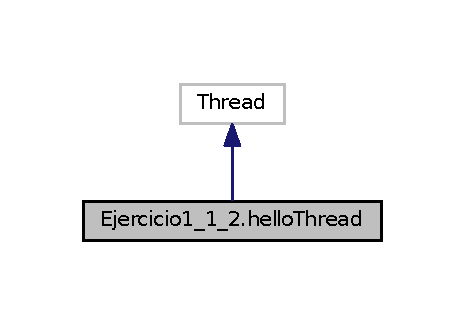
\includegraphics[width=223pt]{class_ejercicio1__1__2_1_1hello_thread__inherit__graph}
\end{center}
\end{figure}


Diagrama de colaboración para Ejercicio1\+\_\+1\+\_\+2.\+hello\+Thread\+:
\nopagebreak
\begin{figure}[H]
\begin{center}
\leavevmode
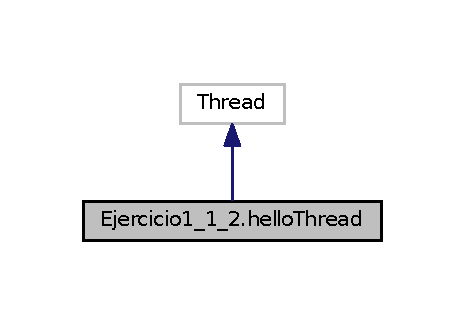
\includegraphics[width=223pt]{class_ejercicio1__1__2_1_1hello_thread__coll__graph}
\end{center}
\end{figure}
\subsection*{Métodos públicos}
\begin{DoxyCompactItemize}
\item 
\hypertarget{class_ejercicio1__1__2_1_1hello_thread_a2bc6e380aaedb4372eda52855fa48437}{}void \hyperlink{class_ejercicio1__1__2_1_1hello_thread_a2bc6e380aaedb4372eda52855fa48437}{run} ()\label{class_ejercicio1__1__2_1_1hello_thread_a2bc6e380aaedb4372eda52855fa48437}

\begin{DoxyCompactList}\small\item\em Función run para iniciar el thread. \end{DoxyCompactList}\end{DoxyCompactItemize}
\subsection*{Métodos públicos estáticos}
\begin{DoxyCompactItemize}
\item 
\hypertarget{class_ejercicio1__1__2_1_1hello_thread_acb76a0580e4cf4015b35bd03dd49cea3}{}static void \hyperlink{class_ejercicio1__1__2_1_1hello_thread_acb76a0580e4cf4015b35bd03dd49cea3}{main} (String\mbox{[}$\,$\mbox{]} args)\label{class_ejercicio1__1__2_1_1hello_thread_acb76a0580e4cf4015b35bd03dd49cea3}

\begin{DoxyCompactList}\small\item\em Función main del ejercicio. \end{DoxyCompactList}\end{DoxyCompactItemize}


\subsection{Descripción detallada}
Creación de hilos usando la clase Thread. 

\begin{DoxyAuthor}{Autor}
Nara, Javier, Esteban 
\end{DoxyAuthor}


La documentación para esta clase fue generada a partir del siguiente fichero\+:\begin{DoxyCompactItemize}
\item 
Ejercicio1\+\_\+1\+\_\+2/hello\+Thread.\+java\end{DoxyCompactItemize}

\hypertarget{class_ejercicio1__1__3_1_1hello_thread___sleep}{}\section{Referencia de la Clase Ejercicio1\+\_\+1\+\_\+3.\+hello\+Thread\+\_\+\+Sleep}
\label{class_ejercicio1__1__3_1_1hello_thread___sleep}\index{Ejercicio1\+\_\+1\+\_\+3.\+hello\+Thread\+\_\+\+Sleep@{Ejercicio1\+\_\+1\+\_\+3.\+hello\+Thread\+\_\+\+Sleep}}


Creación de hilos usando la clase Thread y usando el método sleep para crear el delay de 1 segundo.  




Diagrama de herencias de Ejercicio1\+\_\+1\+\_\+3.\+hello\+Thread\+\_\+\+Sleep
\nopagebreak
\begin{figure}[H]
\begin{center}
\leavevmode
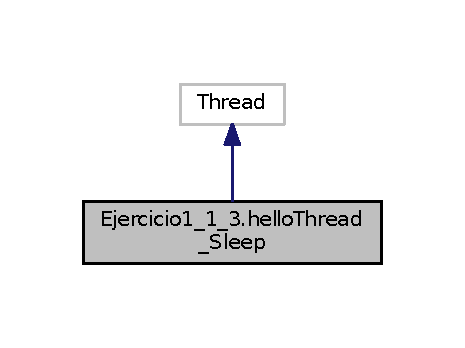
\includegraphics[width=223pt]{class_ejercicio1__1__3_1_1hello_thread___sleep__inherit__graph}
\end{center}
\end{figure}


Diagrama de colaboración para Ejercicio1\+\_\+1\+\_\+3.\+hello\+Thread\+\_\+\+Sleep\+:
\nopagebreak
\begin{figure}[H]
\begin{center}
\leavevmode
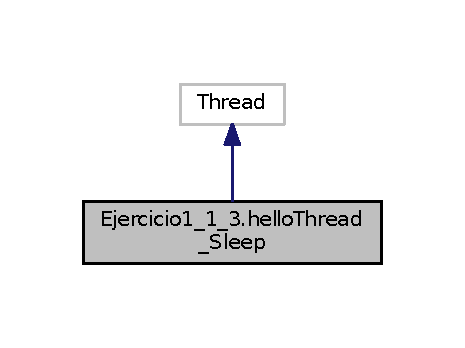
\includegraphics[width=223pt]{class_ejercicio1__1__3_1_1hello_thread___sleep__coll__graph}
\end{center}
\end{figure}
\subsection*{Métodos públicos}
\begin{DoxyCompactItemize}
\item 
\hypertarget{class_ejercicio1__1__3_1_1hello_thread___sleep_ae2d451162bdcec0dfe655a55f03782d9}{}void \hyperlink{class_ejercicio1__1__3_1_1hello_thread___sleep_ae2d451162bdcec0dfe655a55f03782d9}{run} ()\label{class_ejercicio1__1__3_1_1hello_thread___sleep_ae2d451162bdcec0dfe655a55f03782d9}

\begin{DoxyCompactList}\small\item\em Función run para iniciar el thread. \end{DoxyCompactList}\end{DoxyCompactItemize}
\subsection*{Métodos públicos estáticos}
\begin{DoxyCompactItemize}
\item 
\hypertarget{class_ejercicio1__1__3_1_1hello_thread___sleep_aed9e494f20a5978895747a9b78bdde60}{}static void \hyperlink{class_ejercicio1__1__3_1_1hello_thread___sleep_aed9e494f20a5978895747a9b78bdde60}{main} (String\mbox{[}$\,$\mbox{]} args)\label{class_ejercicio1__1__3_1_1hello_thread___sleep_aed9e494f20a5978895747a9b78bdde60}

\begin{DoxyCompactList}\small\item\em Función main del ejercicio. \end{DoxyCompactList}\end{DoxyCompactItemize}


\subsection{Descripción detallada}
Creación de hilos usando la clase Thread y usando el método sleep para crear el delay de 1 segundo. 

\begin{DoxyAuthor}{Autor}
Nara, Javier, Esteban 
\end{DoxyAuthor}


La documentación para esta clase fue generada a partir del siguiente fichero\+:\begin{DoxyCompactItemize}
\item 
Ejercicio1\+\_\+1\+\_\+3/hello\+Thread\+\_\+\+Sleep.\+java\end{DoxyCompactItemize}

\hypertarget{class_ejercicio1__1__4_1_1_runnable___activo}{}\section{Referencia de la Clase Ejercicio1\+\_\+1\+\_\+4.\+Runnable\+\_\+\+Activo}
\label{class_ejercicio1__1__4_1_1_runnable___activo}\index{Ejercicio1\+\_\+1\+\_\+4.\+Runnable\+\_\+\+Activo@{Ejercicio1\+\_\+1\+\_\+4.\+Runnable\+\_\+\+Activo}}


Creación de hilos usando la clase Runnable y usando los metodos active\+Count y current\+Thread para postrar el numero de hilos y el hilo actual.  




Diagrama de herencias de Ejercicio1\+\_\+1\+\_\+4.\+Runnable\+\_\+\+Activo
\nopagebreak
\begin{figure}[H]
\begin{center}
\leavevmode
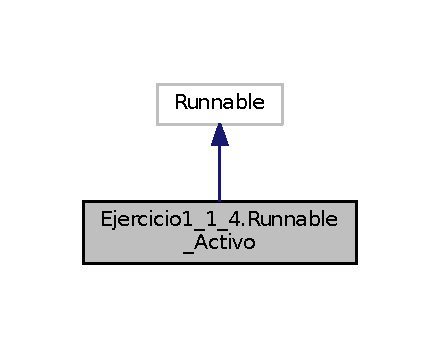
\includegraphics[width=211pt]{class_ejercicio1__1__4_1_1_runnable___activo__inherit__graph}
\end{center}
\end{figure}


Diagrama de colaboración para Ejercicio1\+\_\+1\+\_\+4.\+Runnable\+\_\+\+Activo\+:
\nopagebreak
\begin{figure}[H]
\begin{center}
\leavevmode
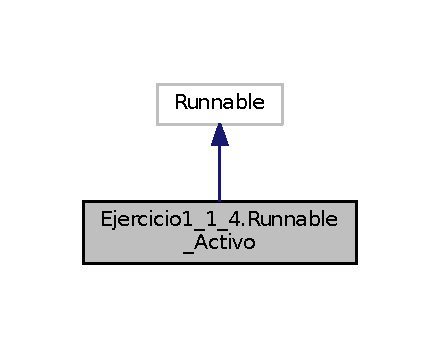
\includegraphics[width=211pt]{class_ejercicio1__1__4_1_1_runnable___activo__coll__graph}
\end{center}
\end{figure}
\subsection*{Métodos públicos}
\begin{DoxyCompactItemize}
\item 
\hypertarget{class_ejercicio1__1__4_1_1_runnable___activo_acba1ef516ab945a02ad45134bf412c24}{}void \hyperlink{class_ejercicio1__1__4_1_1_runnable___activo_acba1ef516ab945a02ad45134bf412c24}{run} ()\label{class_ejercicio1__1__4_1_1_runnable___activo_acba1ef516ab945a02ad45134bf412c24}

\begin{DoxyCompactList}\small\item\em Función run para iniciar el thread. \end{DoxyCompactList}\end{DoxyCompactItemize}
\subsection*{Métodos públicos estáticos}
\begin{DoxyCompactItemize}
\item 
\hypertarget{class_ejercicio1__1__4_1_1_runnable___activo_af6744837b413387636ccc487b8bf54cc}{}static void \hyperlink{class_ejercicio1__1__4_1_1_runnable___activo_af6744837b413387636ccc487b8bf54cc}{main} (String\mbox{[}$\,$\mbox{]} args)\label{class_ejercicio1__1__4_1_1_runnable___activo_af6744837b413387636ccc487b8bf54cc}

\begin{DoxyCompactList}\small\item\em Función main del ejercicio. \end{DoxyCompactList}\end{DoxyCompactItemize}


\subsection{Descripción detallada}
Creación de hilos usando la clase Runnable y usando los metodos active\+Count y current\+Thread para postrar el numero de hilos y el hilo actual. 

\begin{DoxyAuthor}{Autor}
Nara, Javier, Esteban 
\end{DoxyAuthor}


La documentación para esta clase fue generada a partir del siguiente fichero\+:\begin{DoxyCompactItemize}
\item 
Ejercicio1\+\_\+1\+\_\+4/Runnable\+\_\+\+Activo.\+java\end{DoxyCompactItemize}

\hypertarget{class_ejercicio1__1__4_1_1_thread___activo}{}\section{Referencia de la Clase Ejercicio1\+\_\+1\+\_\+4.\+Thread\+\_\+\+Activo}
\label{class_ejercicio1__1__4_1_1_thread___activo}\index{Ejercicio1\+\_\+1\+\_\+4.\+Thread\+\_\+\+Activo@{Ejercicio1\+\_\+1\+\_\+4.\+Thread\+\_\+\+Activo}}


Creación de hilos usando la clase Thread y usando los metodos active\+Count y current\+Thread para postrar el numero de hilos y el hilo actual.  




Diagrama de herencias de Ejercicio1\+\_\+1\+\_\+4.\+Thread\+\_\+\+Activo
\nopagebreak
\begin{figure}[H]
\begin{center}
\leavevmode
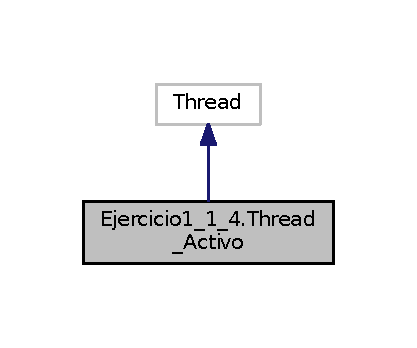
\includegraphics[width=200pt]{class_ejercicio1__1__4_1_1_thread___activo__inherit__graph}
\end{center}
\end{figure}


Diagrama de colaboración para Ejercicio1\+\_\+1\+\_\+4.\+Thread\+\_\+\+Activo\+:
\nopagebreak
\begin{figure}[H]
\begin{center}
\leavevmode
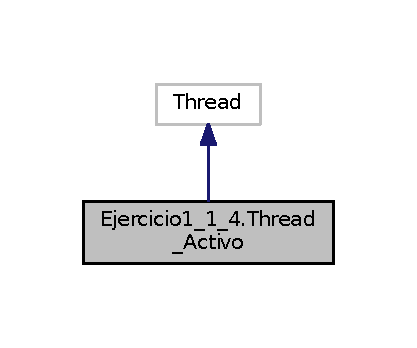
\includegraphics[width=200pt]{class_ejercicio1__1__4_1_1_thread___activo__coll__graph}
\end{center}
\end{figure}
\subsection*{Métodos públicos}
\begin{DoxyCompactItemize}
\item 
\hypertarget{class_ejercicio1__1__4_1_1_thread___activo_abf24f11ac559a1049ce909cb6db4abd8}{}void \hyperlink{class_ejercicio1__1__4_1_1_thread___activo_abf24f11ac559a1049ce909cb6db4abd8}{run} ()\label{class_ejercicio1__1__4_1_1_thread___activo_abf24f11ac559a1049ce909cb6db4abd8}

\begin{DoxyCompactList}\small\item\em Función run para iniciar el thread. \end{DoxyCompactList}\end{DoxyCompactItemize}
\subsection*{Métodos públicos estáticos}
\begin{DoxyCompactItemize}
\item 
\hypertarget{class_ejercicio1__1__4_1_1_thread___activo_ab3e61d53d79ec28d9a95bfabd9661a34}{}static void \hyperlink{class_ejercicio1__1__4_1_1_thread___activo_ab3e61d53d79ec28d9a95bfabd9661a34}{main} (String\mbox{[}$\,$\mbox{]} args)\label{class_ejercicio1__1__4_1_1_thread___activo_ab3e61d53d79ec28d9a95bfabd9661a34}

\begin{DoxyCompactList}\small\item\em Función main del ejercicio. \end{DoxyCompactList}\end{DoxyCompactItemize}


\subsection{Descripción detallada}
Creación de hilos usando la clase Thread y usando los metodos active\+Count y current\+Thread para postrar el numero de hilos y el hilo actual. 

\begin{DoxyAuthor}{Autor}
Nara, Javier, Esteban 
\end{DoxyAuthor}


La documentación para esta clase fue generada a partir del siguiente fichero\+:\begin{DoxyCompactItemize}
\item 
Ejercicio1\+\_\+1\+\_\+4/Thread\+\_\+\+Activo.\+java\end{DoxyCompactItemize}

\hypertarget{class_ejercicio1__3__2_1_1_thread___detenido}{}\section{Referencia de la Clase Ejercicio1\+\_\+3\+\_\+2.\+Thread\+\_\+\+Detenido}
\label{class_ejercicio1__3__2_1_1_thread___detenido}\index{Ejercicio1\+\_\+3\+\_\+2.\+Thread\+\_\+\+Detenido@{Ejercicio1\+\_\+3\+\_\+2.\+Thread\+\_\+\+Detenido}}


Crea un Thread y comprueba con is\+Interrupted() e interrupted() antes y después de interrumpirlo.  




Diagrama de herencias de Ejercicio1\+\_\+3\+\_\+2.\+Thread\+\_\+\+Detenido
\nopagebreak
\begin{figure}[H]
\begin{center}
\leavevmode
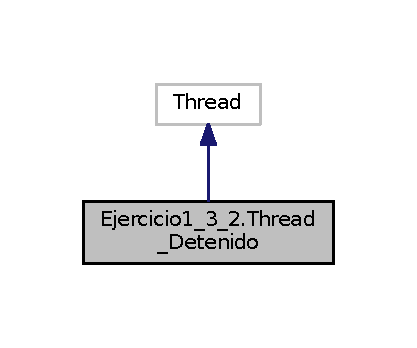
\includegraphics[width=200pt]{class_ejercicio1__3__2_1_1_thread___detenido__inherit__graph}
\end{center}
\end{figure}


Diagrama de colaboración para Ejercicio1\+\_\+3\+\_\+2.\+Thread\+\_\+\+Detenido\+:
\nopagebreak
\begin{figure}[H]
\begin{center}
\leavevmode
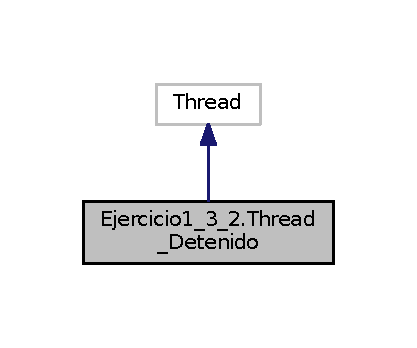
\includegraphics[width=200pt]{class_ejercicio1__3__2_1_1_thread___detenido__coll__graph}
\end{center}
\end{figure}
\subsection*{Métodos públicos}
\begin{DoxyCompactItemize}
\item 
\hypertarget{class_ejercicio1__3__2_1_1_thread___detenido_a6be43334720506b0cc43c8020caef6e8}{}{\bfseries Thread\+\_\+\+Detenido} (int n)\label{class_ejercicio1__3__2_1_1_thread___detenido_a6be43334720506b0cc43c8020caef6e8}

\item 
\hypertarget{class_ejercicio1__3__2_1_1_thread___detenido_a0d8e2160e3d5841b707dec80edf4da66}{}void \hyperlink{class_ejercicio1__3__2_1_1_thread___detenido_a0d8e2160e3d5841b707dec80edf4da66}{run} ()\label{class_ejercicio1__3__2_1_1_thread___detenido_a0d8e2160e3d5841b707dec80edf4da66}

\begin{DoxyCompactList}\small\item\em Función run para iniciar el thread. \end{DoxyCompactList}\end{DoxyCompactItemize}
\subsection*{Métodos públicos estáticos}
\begin{DoxyCompactItemize}
\item 
\hypertarget{class_ejercicio1__3__2_1_1_thread___detenido_ae18c982e481fc76e3d53e6f7220457f2}{}static void \hyperlink{class_ejercicio1__3__2_1_1_thread___detenido_ae18c982e481fc76e3d53e6f7220457f2}{main} (String\mbox{[}$\,$\mbox{]} args)\label{class_ejercicio1__3__2_1_1_thread___detenido_ae18c982e481fc76e3d53e6f7220457f2}

\begin{DoxyCompactList}\small\item\em Función main del ejercicio. \end{DoxyCompactList}\end{DoxyCompactItemize}


\subsection{Descripción detallada}
Crea un Thread y comprueba con is\+Interrupted() e interrupted() antes y después de interrumpirlo. 

\begin{DoxyAuthor}{Autor}
Nara, Javier, Esteban 
\end{DoxyAuthor}


La documentación para esta clase fue generada a partir del siguiente fichero\+:\begin{DoxyCompactItemize}
\item 
Ejercicio1\+\_\+3\+\_\+2/Thread\+\_\+\+Detenido.\+java\end{DoxyCompactItemize}

%--- End generated contents ---

% Index
\backmatter
\newpage
\phantomsection
\clearemptydoublepage
\addcontentsline{toc}{chapter}{Índice}
\printindex

\end{document}
